\documentclass{beamer}

\usepackage{graphicx}
\usepackage{framed}

\begin{document}
%================================================================================= %
\begin{frame}
\begin{figure}
\centering
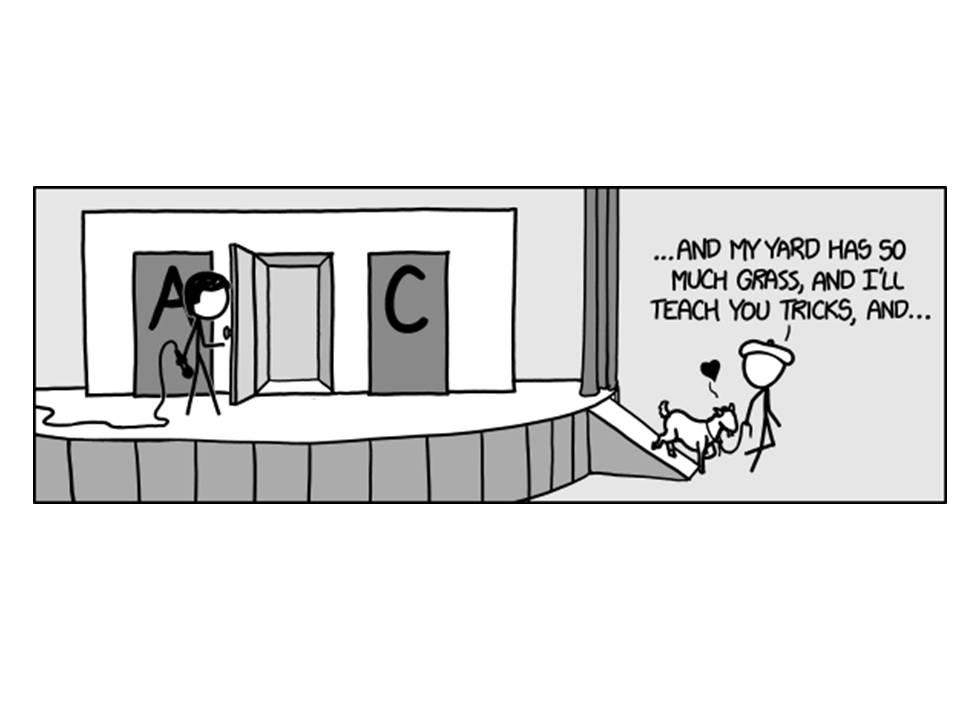
\includegraphics[width=1.1\linewidth]{MontyHall/Slide1}


\end{figure}

\end{frame}
%============================================================================= %
%================================================================================= %
\begin{frame}
	\frametitle{Let's Make a Deal with Monty Hall}
	\begin{figure}
		\centering
		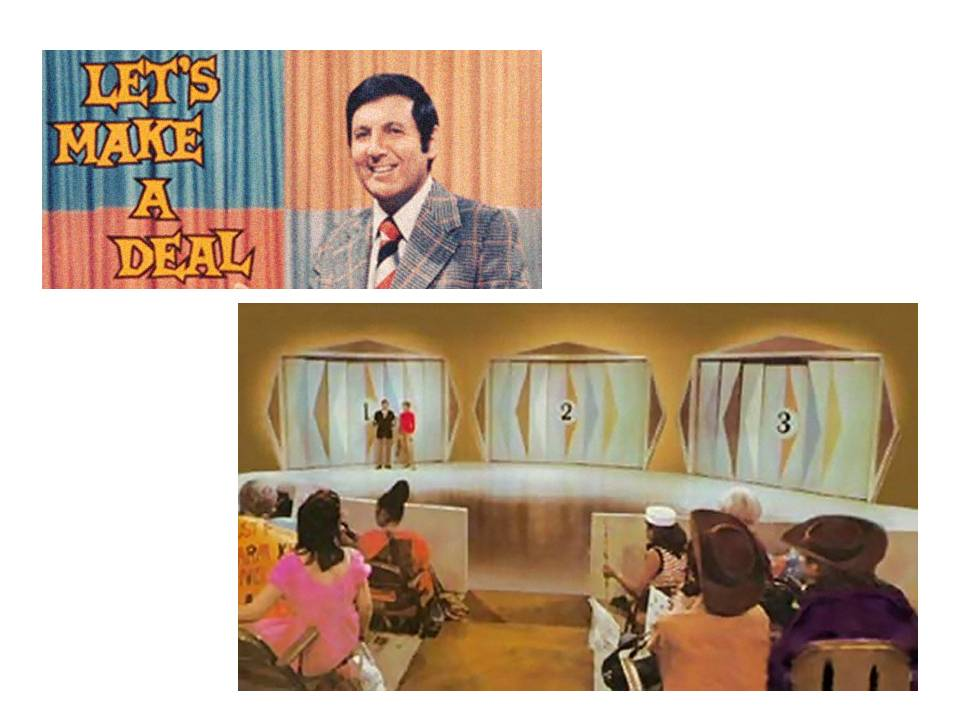
\includegraphics[width=0.99\linewidth]{MontyHall/Slide2}
		
	\end{figure}
	
\end{frame}
%============================================================================= %
\begin{frame}
	
	\frametitle{Monty Hall Problem}\LARGE
	\begin{itemize}
	\item Suppose that there are three closed doors on the set of the  \textbf{\emph{Let's Make a Deal}}, a TV game show presented by Monty Hall. 
	\item Behind one of these doors is a car; behind the other two are goats. 
	\item The contestant does not know where the car is, but Monty Hall does.
	
	\item 
	The contestant selects a door, but not the outcome is not immediately evident. 
	\end{itemize}
	
\end{frame}
%============================================================================ %
\begin{frame}
	
	\frametitle{Monty Hall Problem}\LARGE
	\begin{itemize}
	\item Monty opens one of the remaining ``wrong" doors - revealing a goat.
\end{itemize}

\begin{figure}
\centering
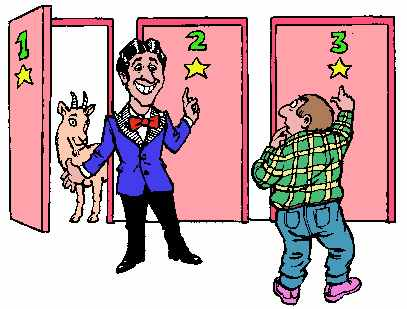
\includegraphics[width=0.7\linewidth]{MontyHall/goat}
\caption{}
\label{fig:goat}
\end{figure}

	{ \Large \textit{Remember this for later : If the contestant has already chosen the correct door, Monty is equally likely to open either of the two remaining doors.}
}
\end{frame}
%============================================================================ %
\begin{frame}
	\frametitle{Monty Hall Problem}\LARGE
	\begin{itemize}
		\item \textbf{Stick or Switch}
	After Monty has shown a goat behind the door that he opens, the contestant is always given the option to switch doors: from the one they have already to select to the other closed door. 
	\item \textbf{Question} -  What is the probability of winning the car if she stays with her first choice? What if she decides to switch?
	\end{itemize}
\end{frame}

%================================================================================= %
\begin{frame}
	\frametitle{Ask Marilyn}
	\begin{figure}
		\centering
		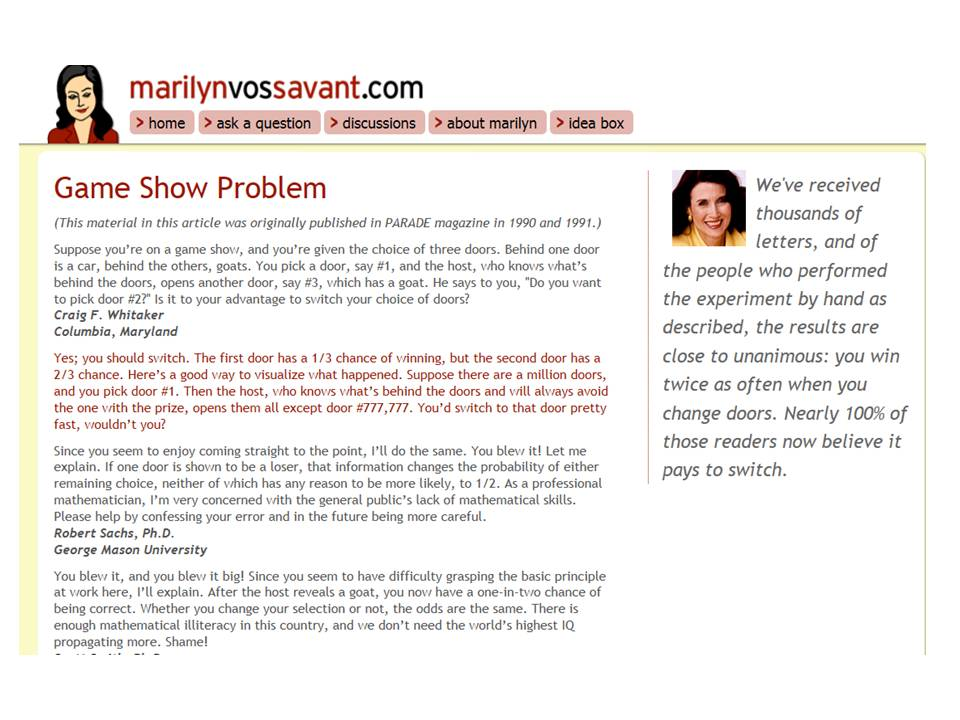
\includegraphics[width=1.17\linewidth]{MontyHall/Slide3}

	\end{figure}
	
\end{frame}
%============================================================================= %

	
	%================================================================================= %
	\begin{frame}
		\frametitle{The Game Show Problem}
		\begin{figure}
			\centering
			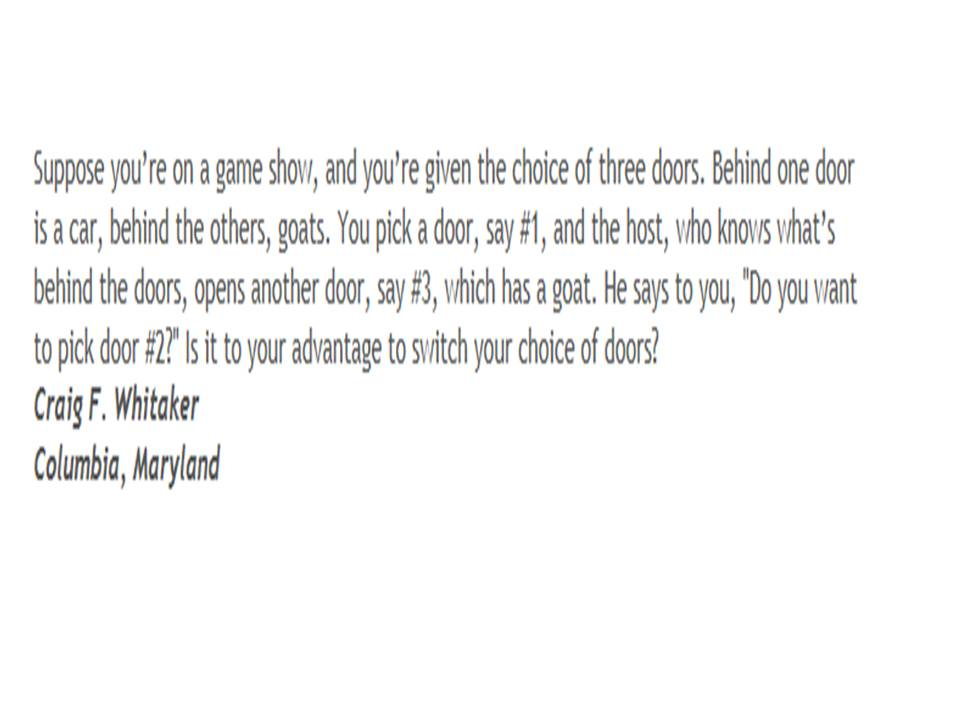
\includegraphics[width=1.1\linewidth]{MontyHall/Slide4}
	
		\end{figure}
		
	\end{frame}
	%============================================================================= %

\begin{frame}
\Large

\textbf{Is it to your advantage to swith your choice of door?}\\ \bigskip
Three possible answers 
\begin{itemize}
\item Yes - Switch Doors \bigskip

\item No - Stick with Your original choice \bigskip

\item Doesn't Matter either way
\end{itemize}
\end{frame}
%================================================================================= %
\begin{frame}
\frametitle{Marilyn Responds}
		\begin{figure}
		\centering
		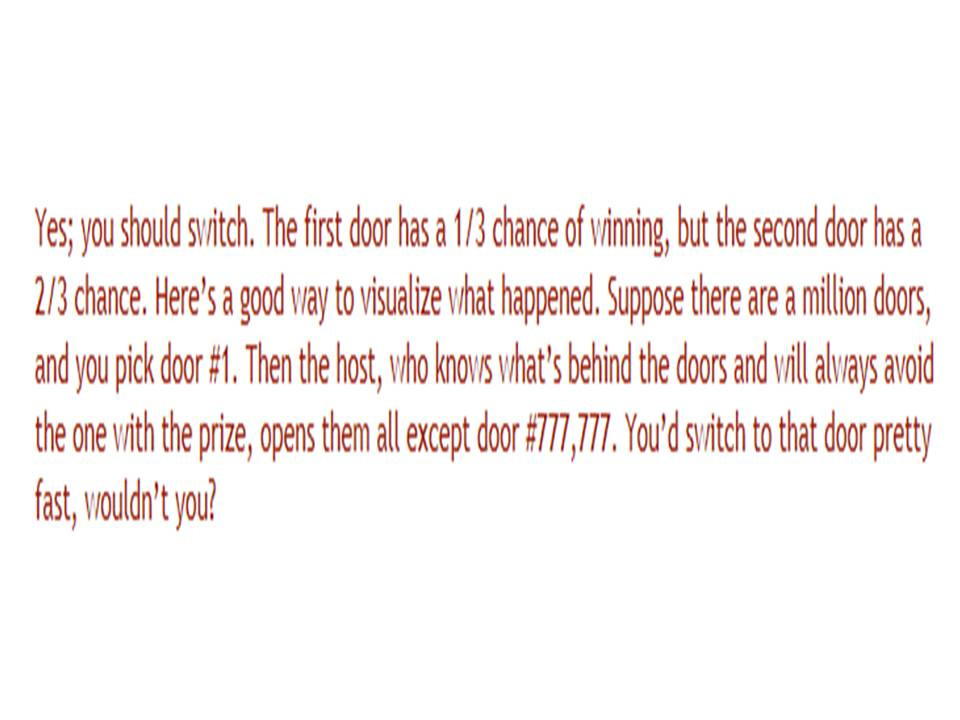
\includegraphics[width=1.0\linewidth]{MontyHall/Slide5}
		
	\end{figure}
		
\end{frame}
%============================================================================= %
\begin{frame}
	\LARGE
	\[ \mbox{and that was the end of that....} \]
	\bigskip
		\LARGE
		\[ \mbox{except....} \]
\end{frame}
%================================================================================= %
\begin{frame}
	\begin{figure}
		\centering
		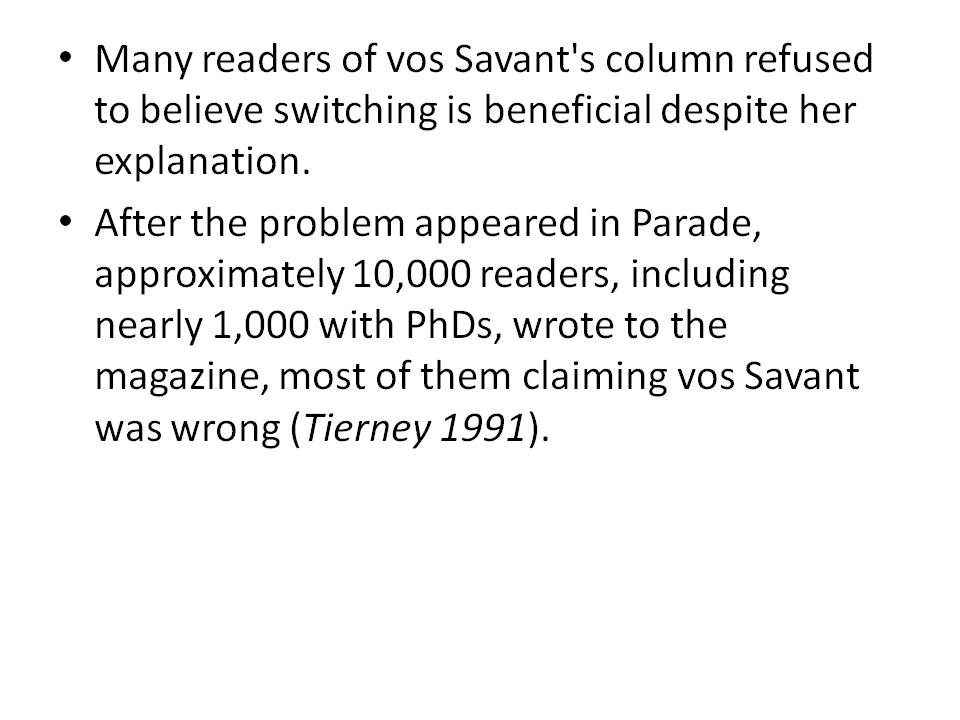
\includegraphics[width=1.1\linewidth]{MontyHall/Slide6}
		
	\end{figure}
	
\end{frame}
%============================================================================= %

%================================================================================= %
\begin{frame}
	
	Let's read some letters!!!!
	\begin{figure}
		\centering
		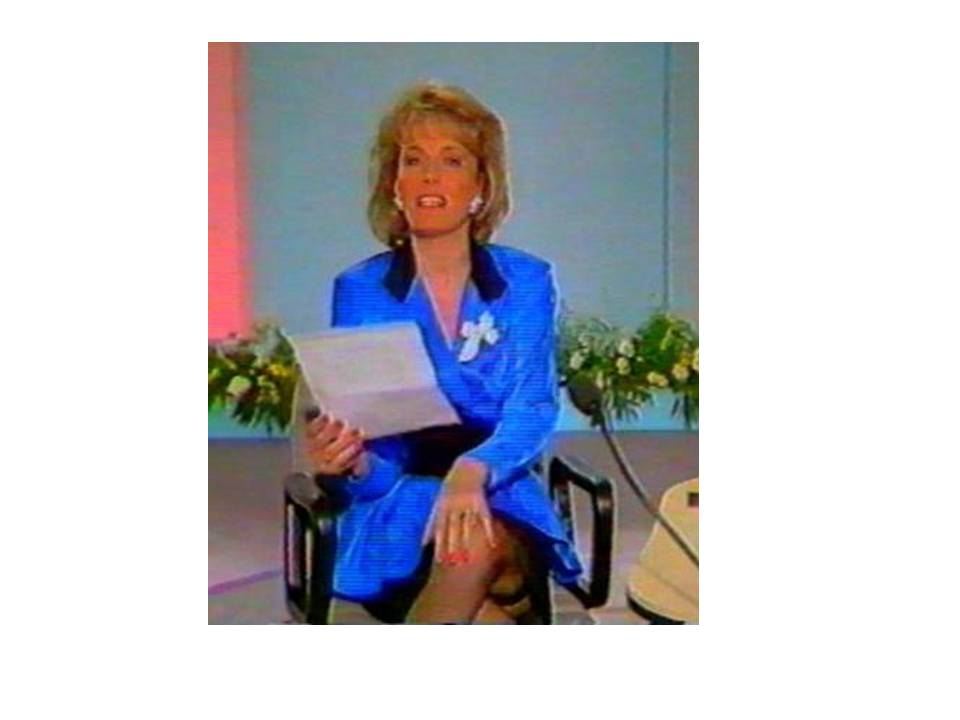
\includegraphics[width=0.9\linewidth]{MontyHall/Slide7}
		\end{figure}
	
\end{frame}

%================================================================================= %
\begin{frame}
	\begin{figure}

		
\includegraphics[width=1.20\linewidth]{MontyHall/Slide8}
		
	\end{figure}
	
\end{frame}
%============================================================================= %

\begin{frame}
	\begin{figure}
		\centering
		
\includegraphics[width=0.7\linewidth]{MontyHall/687}
	\end{figure}
	
\end{frame}
%================================================================================= %
\begin{frame}
	\begin{figure}
		\centering
		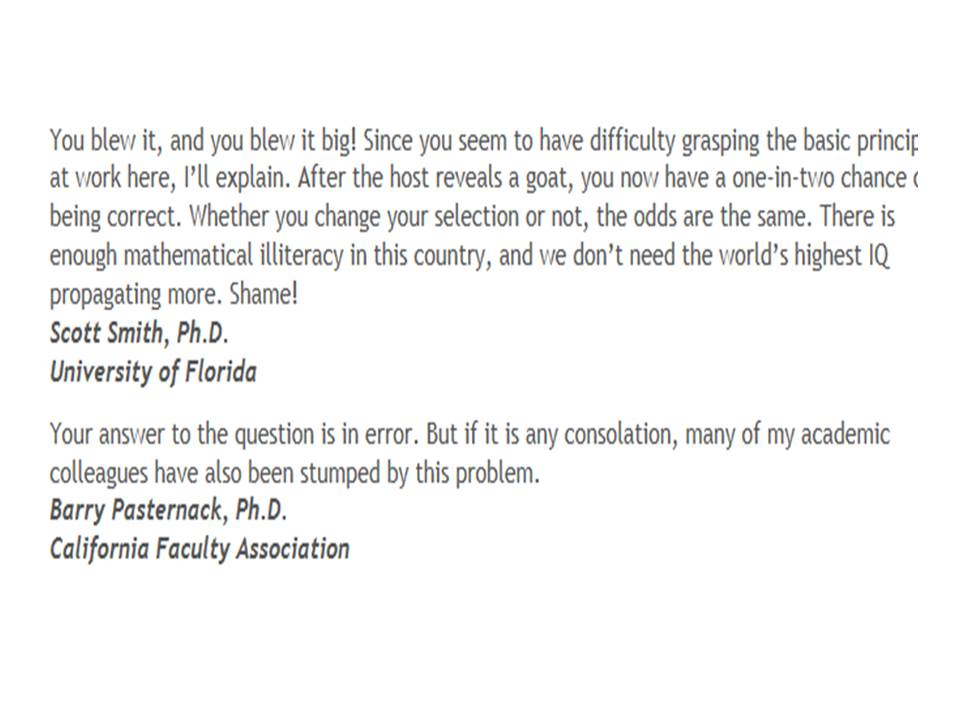
\includegraphics[width=1.1\linewidth]{MontyHall/Slide9}

	\end{figure}
	
\end{frame}
%============================================================================= %


%================================================================================= %
\begin{frame}
	\begin{figure}
		\centering
		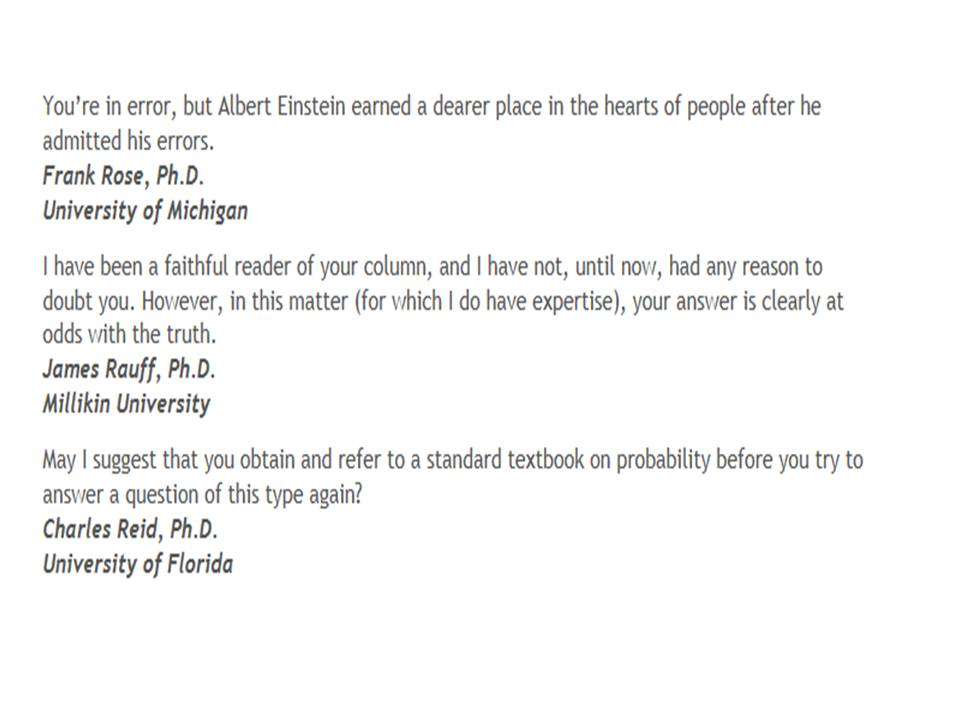
\includegraphics[width=1.16\linewidth]{MontyHall/Slide10}
		
	\end{figure}
	
\end{frame}
%============================================================================= %

%================================================================================= %
\begin{frame}
	\begin{figure}
		\centering
		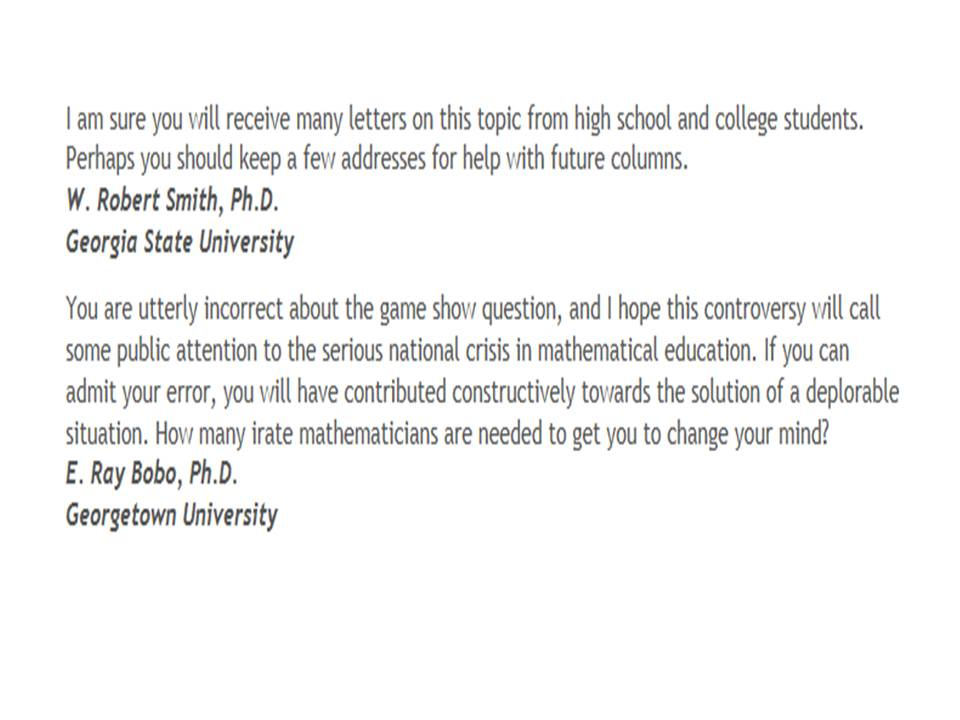
\includegraphics[width=1.17\linewidth]{MontyHall/Slide11}
		
	\end{figure}
	
\end{frame}
%============================================================================= %

%================================================================================= %
\begin{frame}
	\begin{figure}
		\centering
		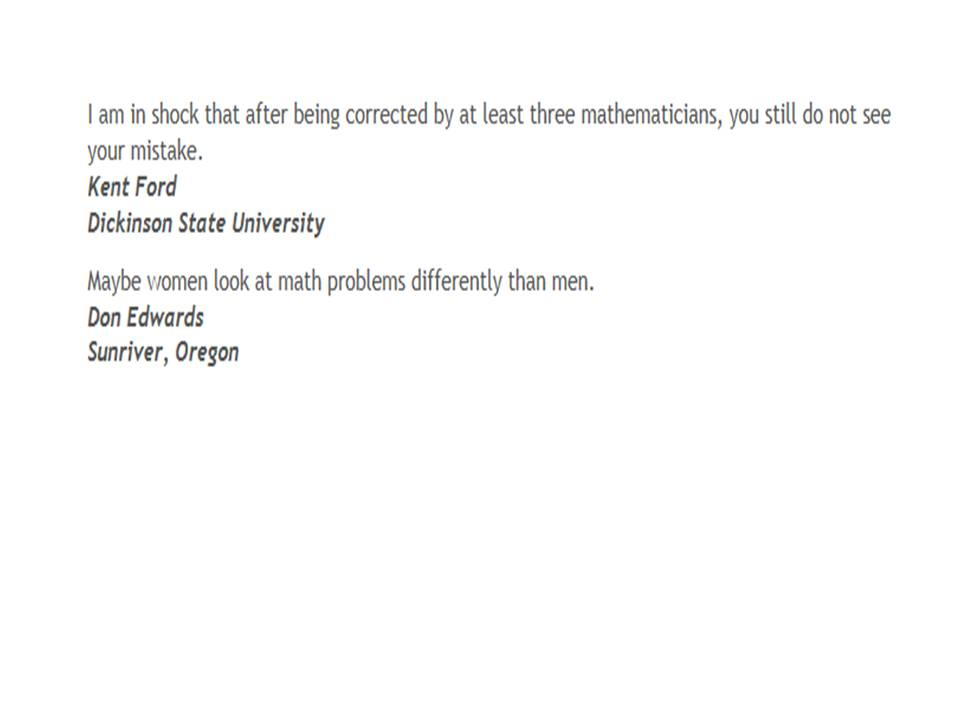
\includegraphics[width=1.18\linewidth]{MontyHall/Slide12}

	\end{figure}
	
\end{frame}
%============================================================================= %

%================================================================================= %
\begin{frame}
	\begin{figure}
		\centering
		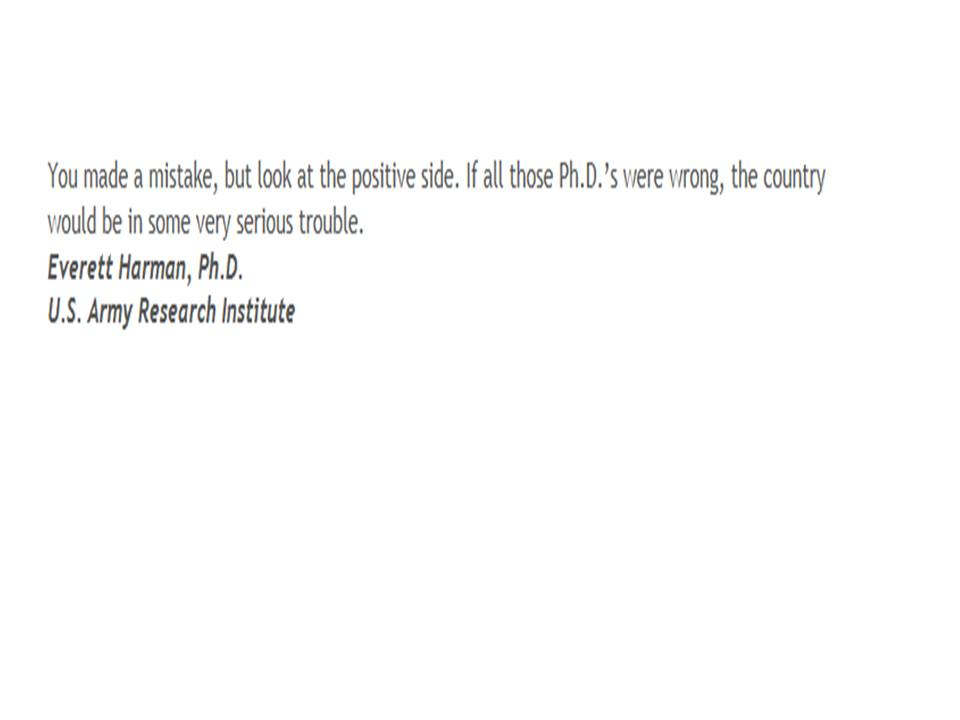
\includegraphics[width=1.16\linewidth]{MontyHall/Slide13}
	\end{figure}
	
\end{frame}
%============================================================================= %
%================================================================================= %
\begin{frame}
	\begin{figure}
		\centering
		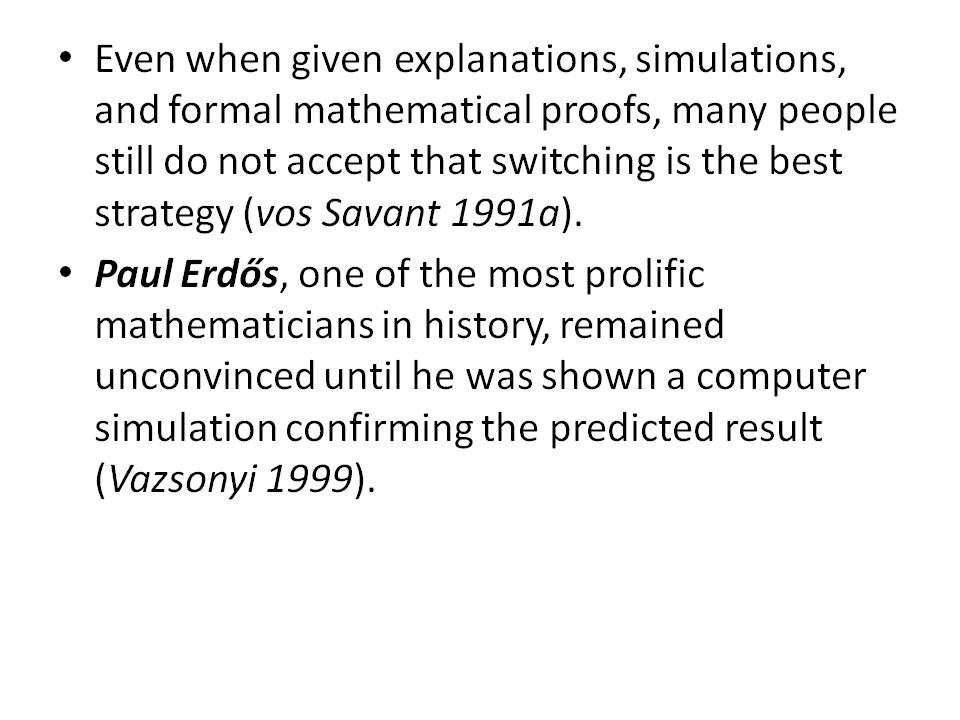
\includegraphics[width=1.17\linewidth]{MontyHall/Slide14}

	\end{figure}
	
\end{frame}
%============================================================================= %

%================================================================================= %
\begin{frame}
	\begin{figure}
		\centering
		
\includegraphics[width=1.17\linewidth]{MontyHall/Slide15}
		
	\end{figure}
	
\end{frame}
%============================================================================= %
%============================================================================ %
\begin{frame}
	
	\frametitle{Implementation with \texttt{R} (part 1)}
	
	\begin{itemize}
\item e have 3 doors to choose from, so we will define a sequence A,B and C. 
\item The command \texttt{\textbf{sample(,n)}} takes a sample of size n from a specified set of values. 
\item Here we just want to select one door to be our "correct door" and another to be ``selected" door (i.e. the contestant selects)
\end{itemize}
	
	
\end{frame}

%============================================================================ %
\begin{frame}[fragile]
	\frametitle{Implementation (part 1)}
	These events are independent. We will perform the selection for both doors separately, but this can be implemented in one command.
	
	
	\begin{framed}
		\begin{verbatim}
		Doors = c("A","B","C")
		Correct = sample(Doors,1)
		Choice = sample(Doors,1)
		\end{verbatim} 
	\end{framed}
\end{frame}
%============================================================================ %
\begin{frame}[fragile]
	A wrong door must be selected to be opened. The door selected by the contestant can't be chosen. First let us select the doors that must stay closed, then find the ones we can choose from to open
	
	\begin{framed}
		\begin{verbatim}
		StayClosed = union(Correct, Choice)
		CanOpen = setdiff(Doors, StayClosed)
		\end{verbatim} 
	\end{framed}
\end{frame}
%============================================================================ %
%============================================================================ %
\begin{frame}[fragile]
	
	\begin{framed}
		\begin{verbatim}
		NotOpen = setdiff(Doors,Open); Stick = Choice        
		#The previous statement is to aid the narrative. 
		
		Switch = setdiff(NotOpen,Choice)
		\end{verbatim} 
	\end{framed}
\end{frame}
%============================================================================ %
%============================================================================ %
\begin{frame}[fragile]
	
	\begin{framed}
		\begin{verbatim}	
		# Was sticking the right decision? Or was switching?
		# The following logicial statements  will tell us.
		
		Stick==Choice ## 1 for Yes 0 for No 
		
		Switch==Choice ## 1 for Yes 0 for No 
		\end{verbatim} 
	\end{framed}
\end{frame}
\end{document}
%============================================================================ %
\begin{frame}[fragile]
	
	\frametitle{Writing a Function}
	We are going to create a function \texttt{\textbf{MHfunc()}} to help us simulate a solution for the Monty Hall Problem. The function is constructed using \texttt{R} code we have seen already. The output of the function is returned as a data frame, with three columns:
	\begin{description}
		\item[Correct] : The number of the correct door.
		\item[Choice] :  The door that the contestant chose originally, and the door selected if the contestant decided to ``stick".
		\item[Switch] : The door selected if the contestant chose to ``switch".
	\end{description}
\end{frame}

\end{document}
